\documentclass{article}
\usepackage{graphicx}
\usepackage{geometry}
\geometry{a4paper, portrait, margin=0.9in}


\begin{document}
\begin{titlepage}
   \vspace*{\stretch{3.0}}
   \begin{center}
      \Large\textbf{CTARA Koregaon Project 2016}\\
      
      \large\textbf{Prof. Vikram M. Gadre}
      
      \large\textit{Sarthak Jain 12D110043}
      \\
      \large\textit{Abhishek Khadiya 131030001}
      \\
      \large\textit{Koustubh Dwivedy 140010016}
      \\
      \large\textit{Swadesh Singh 130020088}
      \\
      \large\textit{Preshit Gulgulia 130040070}
      \\
      \large\textit{Angothu Prasanna 130070055}
   \end{center}
   \vspace*{\stretch{3.0}}
\end{titlepage}

\tableofcontents

\newpage
\section{Introduction}
Over the Academic Year 2015-16, two TDSL (Technology and Development Supervised Learning) teams have contributed to the development of the village of Koregaon near Satara, based on a nearby village named Kapshi. This TDSL effort intends to continue that endeavour.

\subsection{Location}
Koregaon village is located in the Satara district at distance of 45 km from Satara town and is 90km
south of Pune. Village lies in the leeward side of Mahadeo hills.
\begin{figure}[h]
\begin{center}
  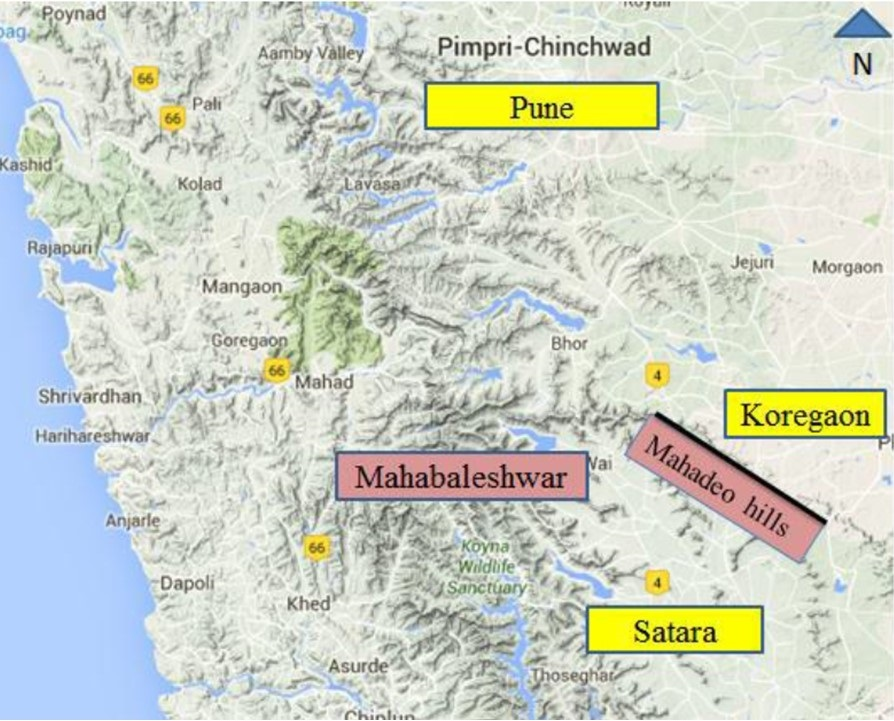
\includegraphics[scale=0.4]{images/location.jpg}
\end{center}
\end{figure}

\subsection{Project Description}
The aim of this project is to bring overall development of the Koregaon village. This village suffers from
water shortage which affects their agricultural production which is mostly onion. It was found that the
village does not have any onion storage facility. Past year's team worked on developing infrastructure to solve the problem of onion storage. Our team's aim is to deal with the problem of water shortage.
\section{Situation Review}
Koregaon village is one the most badly drought affected areas. The annual rainfall at the place is quite minimal and is hardly sufficient for the people to meet their demands. The situation is even worsened during the summers. While regions like Mahableshwar which are close to Sahayadri hills in west, receive rainfall as high as 2223 mm, moving eastwards the rainfall amount drops to less than 900 mm in the Taluka of Koregaon, Karad,Satara and to less than 600 mm in the Taluka of Man, Khatav, Phaltan and Khandala.
\subsection{Dependence on Monsoon Rains}
Currently Koregaon is dependent heavily on the monsoon rain. There are two small seasonal streams which run besides the village. There is small lake just outside the village which was constructed by government in 1960’s when the entire district was under severe drought. This small lake doesn’t have a good catchment area and with poor rainfall it gets dry within few months after monsoon season. Government had constructed two Bandharas (stop dams) on one of the stream but those failed within a year of operation. There are number of wells along the stream. These wells are dug to store the percolated water from stream. However due to rocky terrain the percolation is poor in these wells. So the villagers have put a bore well to meet the need of water. But this is leading to continuous decrease in the level of water table.

Looking at the much higher construction cost for the canal, the option to electrically pump the water from the stream to the lake seems to be significantly cheaper and feasible. In order to select the specifications of the pump we will visit the place and look at the geographical features of the area of interest. The lake existing in the village is very shallow and due to high temperature conditions in summer, the evaporation losses are significant since most of the surface areas is exposed to sun due to less depth.

The water collected in this lake would come from a nearby stream that remains dry for most of the year but fills up during the rainy season. The proposed solution is to transfer the water from the stream to the lake through pump.

\section{Field Visit I}
\subsection{Field Visit Description}
As our maiden visit to Koregaon, our main objectives were
\begin{itemize}
  \item To observe the problems regarding water shortage, storage facility in the vicinity
  \item To acknowledge the work done till now and support the continuance of it
  \item To propose/validate solutions pertaining especially to water shortage
\end{itemize}
We were able to meet all the main stakeholders regarding this project, and went through all the sites that would serve in the proposed solution.

\subsection{Current Water Facility}
Koregaon Tank Capacity = 25,000 litres
\\
Water required per day = 12,500 litres
\\
This requirement is fulfilled by transference of water from well to the tank. Current Pump specifications to transfer water from the well to storage tank.
\\
Pump capacity = 5 HP
\\
Pipe specification = 3’’ Diameter
\\
Therefore every day the aforementioned pump is used for an hour to meet the daily water requirements.

\subsection{Work Accomplished till date}
\begin{itemize}
\item Near completion of storage facility for onions
\item An area of the dam has been dug out to facilitate storage of water
\end{itemize}

\begin{figure}[h]
\begin{center}
  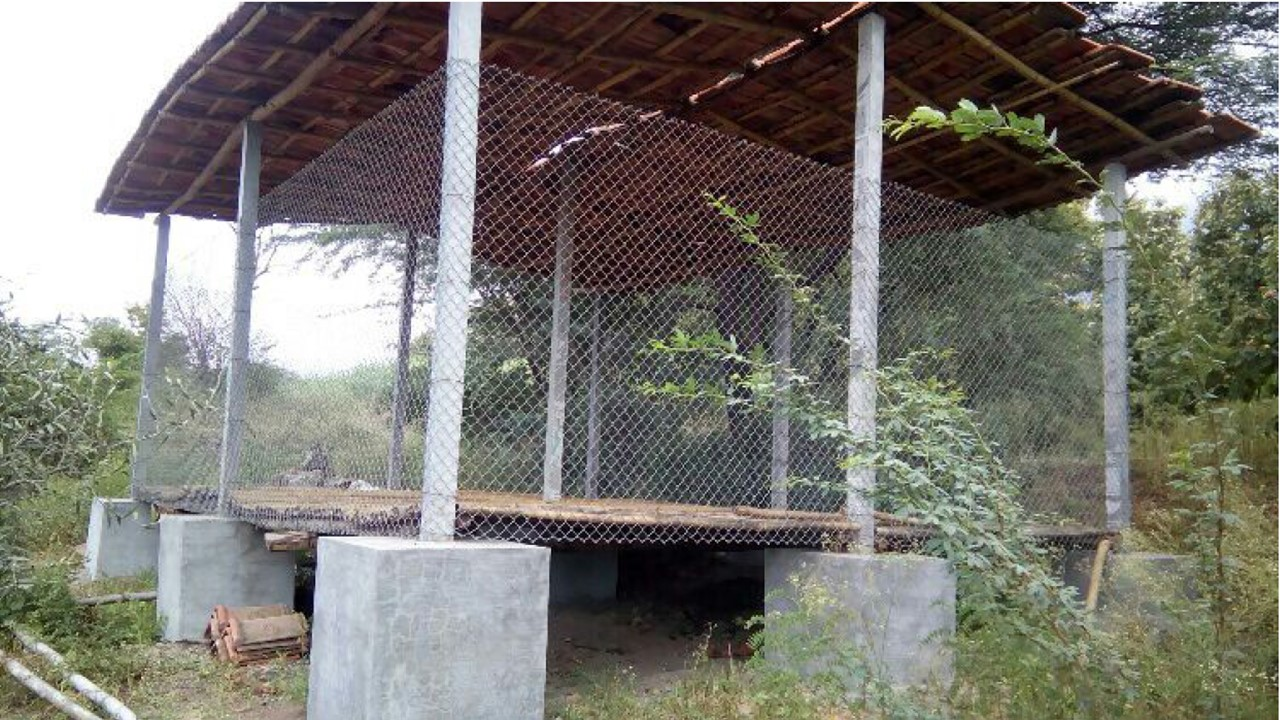
\includegraphics[scale=0.4]{images/onion_storage.jpg}
  \\
  Storage Facility of Onions
\end{center}
\end{figure}

\begin{figure}[h]
\begin{center}
  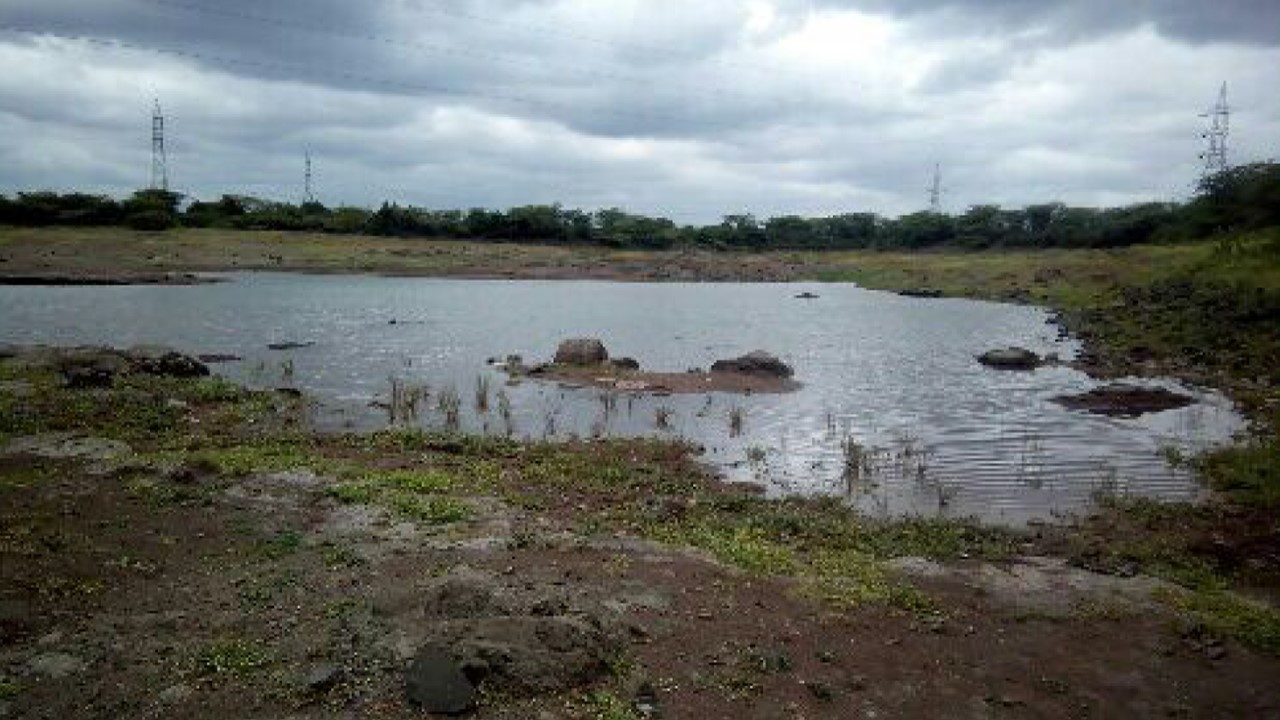
\includegraphics[scale=0.4]{images/dam.jpg}
  \\
  Dam to be filled by stream
\end{center}
\end{figure}

\subsection{The Problem}
During the summer season, the well dries up, generating shortage of drinking water and for irrigation for the villagers. Over the years, the groundwater level has also gone down adding to the above problem.

\subsection{Proposed Solution}
Water to be shifted from the nearby stream to the dam during monsoon season considering
that the water flows in the stream for 2 months to solve following objectives
\begin{itemize}
\item Fill the dam well enough that could be served as the major water source during drought conditions
\item Increase the well water level via percolation through dam
\item Make water available for irrigation purposes
\end{itemize}
\underline{5HP Pump and 3'' Pipe}\\
Let the pump run for 10 hours/day for these 2 months. So the total water stored in these 2 months is equal to 20 months water requirement of the village. So 5HP pump is sufficient to meet the 1 year eater requirement of the village, considering evaporation of water, percolation, leak losses, etc. Still there is scope to increase the duration of the pump from 10 hrs to 15 hrs, making the total storage to 30 months.
\underline{10HP Pump with 4'' Pipe}\\
We don't think there is a need of a higher pump capacity. But considering the request of the people from Koregaon, we can go at most for this pump.

Requirement of \underline{15 HP Pump and 5'' Pipe} seems unfeasible due to following reasons:
\begin{itemize}
\item Almost double cost of pipes due to increment of diameter
\item Increased cost of pump
\item Higher maintenance required
\end{itemize}

\subsection{Further recommendation}
We also believe that the success of this project will highly
depend on the participation from the people of Koregaon, as it involves high monetary input and maintenance after implementation. We should make sure that all the stakeholders are actively involved and contribute (monetary or otherwise) towards this, to make it possible.

\end{document}